\documentclass[a4paper, 12pt]{article}
\usepackage[top=1cm, bottom=1cm, left=1.5cm, right=1.5cm]{geometry}
\usepackage{pgfplots}
\usepackage[table]{xcolor}


\begin{document}
	\begin{center}
		Universidade Federal do Rio Grande do Norte
		
		Departamento de Engenharia da Computação e Automação
		
		DCA3703 - Programação Paralela
		
		\textbf{Tarefa 1 - Memória Cache}
		
		\textbf{Aluno:} Daniel Bruno Trindade da Silva
	\end{center}
	
	\vspace{0,5cm}
	
	\textbf{Introdução:}
	
	Nesta tarefa, exploramos a multiplicação de matriz por vetor (MxV), com o objetivo de analisar como dois diferentes padrões de acesso aos valores da matriz (por linhas e por colunas) impactam no tempo de execução e o motivo pelo qual as execuções diferem.
	
	
	A tarefa consiste em implementar duas versões do algoritmo em C: uma que percorre a matriz por linhas (com laço externo sobre as linhas e interno sobre as colunas) e outra que percorre por colunas (com laço externo sobre as colunas e interno sobre as linhas). Ao executar ambas as versões faremos a medição de tempo, com o fim de comparar o desempenho das duas abordagens em matrizes de diferentes tamanhos, identificando a partir de qual dimensão os tempos de execução passam a divergir significativamente.
	
	\vspace{0,5cm}
	
	\textbf{Implementação:}
	
	Para testar as duas abordagens e obter seus resultados em um único código, implementamos uma função para cada uma delas: \texttt{mat\_vec\_row}, que realiza o acesso aos elementos da matriz por linhas, e \texttt{mat\_vet\_col}, que acessa os elementos por colunas. Essa estrutura permite testar ambas as abordagens em uma única execução.
	
	Executaremos ambas as funções dentro de um laço de repetição, aumentando progressivamente o número de elementos da matriz e do vetor, a fim de identificar a partir de qual dimensão ocorre uma grande divergência no tempo de execução
	
	Para execução da análise, realizamos a multiplicação da matriz com tamanho \textit{n$\times$n} por um vetor também de tamanho \textit{n} com \textit{n} assumindo os valores de 100, 1000, 10000, 50000 e 100000. Em cada uma das execuções são medidos os tempos de tomados por cada uma das abordagens propostas e entregues em segundos.
	
	\vspace{0,5cm}
	
	\textbf{Código:}
	
	O código utiliza a biblioteca \texttt{stdlib.h} para alocação de memória e a \texttt{time.h} para aferição do tempo de execução. O código ficou como se segue:
	
	
	\begin{verbatim}
		#include <stdio.h>
		#include <stdlib.h>
		#include <time.h>
		
		// Função para medir o tempo
		double get_time(clock_t start, clock_t end) {
			return (double)(end - start) / CLOCKS_PER_SEC;
		}
		
		// Multiplicacao MxV com acesso por linhas
		void mat_vec_row(double** mat, double* vec, double* res, int n) {
			for (int i = 0; i < n; i++) {
				res[i] = 0.0;
				for (int j = 0; j < n; j++) {
					res[i] += mat[i][j] * vec[j];
				}
			}
		}
		
		// Multiplicacao MxV com acesso por colunas
		void mat_vec_col(double** mat, double* vec, double* res, int n) {
			for (int j = 0; j < n; j++) {
				for (int i = 0; i < n; i++) {
					res[i] += mat[i][j] * vec[j];
				}
			}
		}
		
		int main() {
			int sizes[] = {100, 500, 1000, 2000, 3000};
			int num_tests = 5;
			
			for (int t = 0; t < num_tests; t++) {
				int n = sizes[t];
				printf("Tamanho da matriz: %d\n", n);
				
				// Alocação de matriz e vetores
				double** mat = (double**) malloc(n * sizeof(double*));
				double* vec = (double*) malloc(n * sizeof(double));
				double* res_row = (double*) calloc(n, sizeof(double));
				double* res_col = (double*) calloc(n, sizeof(double));
				
				for (int i = 0; i < n; i++) {
					mat[i] = (double*) malloc(n * sizeof(double));
					for (int j = 0; j < n; j++) {
						mat[i][j] = (double)rand() / RAND_MAX;
					}
					vec[i] = (double)rand() / RAND_MAX;
				}
				
				// Tempo para acesso por linhas
				clock_t start = clock();
				mat_vec_row(mat, vec, res_row, n);
				clock_t end = clock();
				printf("Tempo (acesso por linhas): %.4f s\n", get_time(start, end));
				
				// Tempo para acesso por colunas
				start = clock();
				mat_vec_col(mat, vec, res_col, n);
				end = clock();
				printf("Tempo (acesso por colunas): %.4f s\n\n", get_time(start, end));
				
				// Liberação de memória
				for (int i = 0; i < n; i++) {
					free(mat[i]);
				}
				free(mat);
				free(vec);
				free(res_row);
				free(res_col);
			}
			
			return 0;
		}
		
	\end{verbatim}
	
	
	\textbf{Resultados:}
	
	Após execução do código obtivemos os seguintes resultados:
	
	\begin{table}[ht]
		\centering
		\begin{tabular}{|c|c|c|}
			\hline
			\textbf{valor de \textit{n}} & \textbf{Tempo de execução por linhas} & \textbf{Tempo de execução por colunas}  \\
			\hline
			100 & 0,0002s & 0,0002s \\
			500 & 0,0045s & 0,0085s \\
			1.000 & 0,0094s & 0,0215s \\
			5.000 & 0,0940s & 0,3941s \\
			10.000 & 0,3517s & 2,1709s \\
			15.000 & 0,7934s & 6,1648s \\
			\hline
		\end{tabular}
		\caption{Tempo de Execução para cada valor de \textit{n}}
	\end{table}
	
	Como é possível observar, o tempo de execução na abordagem por coluna, se torna muito superior ao da abordagem por linhas. Inicialmente com \textit{n = 500} o tempo da versão por colunas já é quase o dobro do tempo da por linhas. No último teste realizado com \textit{n = 15.000} o tempo usado pelo função que percorre as colunas é quase 8 vezes o tempo usado pela execução por linhas. Podemos observar melhor esse comportamento no seguinte gráfico:
	
	\begin{figure}[h!]
		\centering
		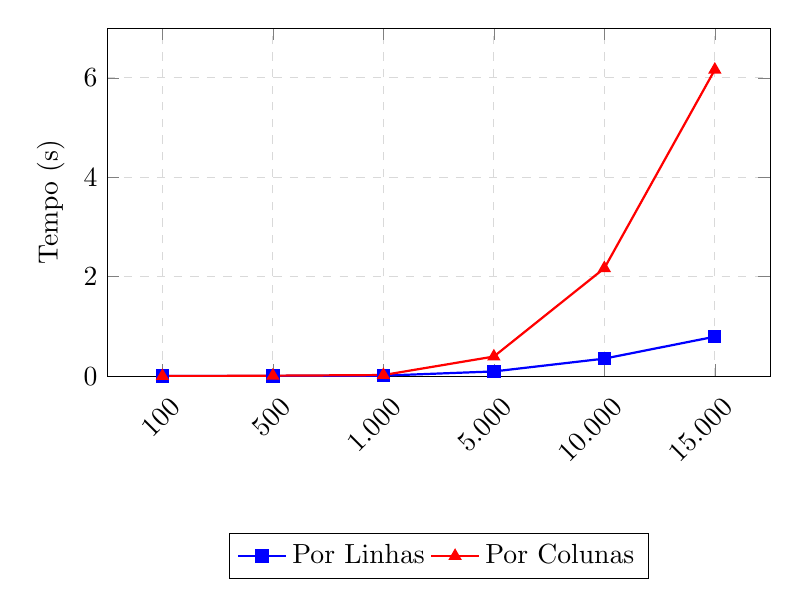
\begin{tikzpicture}
			\begin{axis}[
				width=10cm, height=6cm,
				xlabel={Valor de $n$},
				xlabel style={yshift=-20pt},
				ylabel={Tempo (s)},
				grid=both,
				grid style={dashed, gray!30},
				legend style={at={(0.5,-0.45)}, anchor=north, legend columns=2},
				x tick label style={rotate=45, anchor=east, yshift=-10pt},
				ymin=0, ymax=7,
				ymajorgrids=true,
				xtick=data,
				symbolic x coords={100, 500, 1.000, 5.000, 10.000, 15.000},
				]
				
				% Tempo de execução por linhas (Curva Azul)
				\addplot[
				color=blue,
				mark=square*,
				thick,
				] coordinates {
					(100, 0.0002)
					(500, 0.0045)
					(1.000, 0.0094)
					(5.000, 0.0940)
					(10.000, 0.3517)
					(15.000, 0.7934)
				};
				\addlegendentry{Por Linhas}
				
				% Tempo de execução por colunas (Curva Vermelha)
				\addplot[
				color=red,
				mark=triangle*,
				thick,
				] coordinates {
					(100, 0.0002)
					(500, 0.0085)
					(1.000, 0.0215)
					(5.000, 0.3941)
					(10.000, 2.1709)
					(15.000, 6.1648)
				};
				\addlegendentry{Por Colunas}
				
			\end{axis}
		\end{tikzpicture}
		\caption{Comparação do Tempo de Execução por Linhas e por Colunas}
	\end{figure}
	
	O comportamento observado e essa discrepância na diferença do tempo de execução entre as duas abordagens, se deve a forma com que o sistema lida com o acesso às informações que estão armazenadas no computador, a chamada hierarquia de memória.
	
	A hierarquia de memória de um computador organiza diferentes tipos de memória em níveis, levando em conta sua velocidade, capacidade, custo e proximidade do processador. O objetivo dessa hierarquia é equilibrar desempenho e custo, garantindo acesso rápido aos dados mais utilizados enquanto mantém um armazenamento de longo prazo eficiente.
	
	Para isso funcionar, foram estabelecidos os princípios da temporalidade e da localidade que funcionam da seguinte forma:
	
	
	\textbf{Temporalidade:} Se um dado ou instrução foi acessado recentemente, é provável que seja acessado novamente em breve. Isso ocorre porque loops e variáveis frequentemente reutilizadas são comuns em programas.
	
	\textbf{Localidade:} Se um dado foi acessado, é provável que dados próximos a ele também sejam acessados logo em seguida. Isso acontece porque variáveis e instruções geralmente estão armazenadas de forma contígua na memória, ou seja sequencial.
	
	
	Um outro conhecimento que é necessário para entender o que acontece é saber que o processador trabalha apenas com as informações que estão armazenadas na memória cache. Sempre que o processador precisa de uma informação que não está na memória cache, ele vai fazer uma solicitação para buscar essa informação na memória RAM. Essa busca é feita obedecendo os princípios mencionados, ou seja, a localidade e temporalidade, sendo enviado assim à memoria cache uma linha de dados mais próximos ao dado que foi solicitado.
	
	\vspace{0,5cm}
	
	No nosso experimento, foi observada o seguinte:
	
	\vspace{0,5cm}
	
	Os valores de nossa matriz foram armazenados na RAM de forma contígua como por exemplo:
	
	\begin{table}[ht]
	\centering
	    \begin{tabular}{|c|c|c|c|c|c|c|c|c|}
			\hline
			0x1000 & 0x1004 & 0x1008 & 0x100C & 0x1010 & 0x1014 & 0x1018 & 0x101C & 0x1020 \\
			\hline
			1      & 2      & 3      & 4      & 5      & 6      & 7      & 8      & 9      \\
			\hline
		\end{tabular}
	\caption{Exemplo de armazenamento na memória RAM}
	\end{table}
	
	Ao resgatar o valor de um elemento da primeira linha da matriz, obedecendo o princípio da localidade é também enviado para a memória cache os valores vizinhos o que para a abordagem do acesso por linha é muito bom pois dá celeridade ao processo uma vez que as linhas são armazenadas sequencialmente na memória, isso diminuirá o número de solicitações de leitura em uma memória de acesso mais lento.
	
	\begin{table}[ht]
	\centering
		\begin{tabular}{|c|c|c|c|c|c|c|c|c|}
			\hline
			0x1000 & 0x1004 & 0x1008 & 0x100C & 0x1010 & 0x1014 & 0x1018 & 0x101C & 0x1020 \\
			\hline
			\cellcolor{cyan}1      & \cellcolor{cyan}2      & \cellcolor{cyan}3      & 4      & 5      & 6      & 7      & 8      & 9      \\
			\hline
		\end{tabular}
		\caption{Exemplo de acesso à memória RAM na abordagem por linhas}
	\end{table}
	
	 Já para o acesso aos valores pela abordagem por colunas o computador é obrigado a fazer saltos na leitura, ou seja, em nosso exemplo, obedecendo o princípio da localidade ao resgatar o primeiro valor da primeira linha é enviado a cache os valores 1, 2, e 3, mas nosso programa vai pedir pelo primeiro elemento da segunda linha, causando assim um miss e fazendo com que o processador precise fazer mais buscas na memória RAM, e consequentemente causando a lentidão observada
	
	\begin{table}[ht]
	\centering
		\begin{tabular}{|c|c|c|c|c|c|c|c|c|}
			\hline
			0x1000 & 0x1004 & 0x1008 & 0x100C & 0x1010 & 0x1014 & 0x1018 & 0x101C & 0x1020 \\
			\hline
			\cellcolor{cyan}1      & 2      & 3      & \cellcolor{cyan}4      & 5      & 6      & \cellcolor{cyan}7      & 8      & 9      \\
			\hline
		\end{tabular}
	\caption{Exemplo de acesso à memória RAM na abordagem por colunas}
	\end{table}
	
	\vspace{0,5cm}
	
	\textbf{Conclusão:}
	
	Para os desenvolvedores, compreender o funcionamento do processador e da hierarquia de memória é essencial para otimizar o desempenho dos programas. Como demonstrado neste experimento, a escolha do padrão de acesso aos dados pode ter um impacto significativo na eficiência da execução.


	
	
\end{document}